\documentclass[a4paper, 13pt]{report}
\usepackage[utf8]{inputenc}
\usepackage[a4paper,hmargin={3cm,2.5cm},vmargin={2.5cm,2.5cm}]{geometry}
\usepackage{tikz}
\usepackage{amsmath}
\usetikzlibrary{calc}

\begin{document}
\begin{titlepage}
%\AddToShipoutPictureBG{%

\begin{tikzpicture}[overlay,remember picture]
\draw[line width=4pt]
    ($ (current page.north west) + (2cm,-2cm) $)
    rectangle
    ($ (current page.south east) + (-1cm,2cm) $);
\draw[line width=1.5pt]
    ($ (current page.north west) + (2.2cm,-2.2cm) $)
    rectangle
    ($ (current page.south east) + (-1.2cm,2.2cm) $);
\end{tikzpicture}
\begin{center}
    \textup{\large \textbf{HANOI UNIVERSITY OF SCIENCE AND TECHNOLOGY}\\[0.5cm]\textbf{SCHOOL OF ELECTRONICS AND TELECOMMUNICATIONS}}\\[1cm]
%Title page figure
\end{center}
\begin{center}
\begin{figure}[h]  %h means here other options t , b, p, etc.
\centering
\includegraphics[width=0.2\linewidth]{./BVP-logo bk-rgb.jpg}\\[1cm]
\end{figure}
\textup{\large  PROJECT REPORT\\[1cm]}
\begin{LARGE}
{\textbf {"TELECOMMUNICATION SYSTEMS" }}\end{LARGE}\\[3cm]
\textit{SUBMITTED BY GROUP NUMBER}\\[0.5cm]
\begin{large}
\begin{tabular}{ c c c }
 Bui Huy Hoang & 20172568 & DTVT.07 \\[0.4cm] 
 Nguyen Van Hoang & 20172579 & DTVT.07 \\ [0.4cm] 
 Vu Duc Thai & 20170000 & DTVT.08 \\ [0.4cm]  
\end{tabular}\\[1cm]
\end{large}
\textit{UNDER THE GUIDANCE OF}\\[0.7cm]
\textbf{(Academic Year: 2020-2021)}
\vfill
\end{center}
\end{titlepage}

\pagenumbering{roman}
\setcounter{page}{1}
\newpage
\tableofcontents
\listoffigures
\listoftables



% \maketitle
\newpage
\pagenumbering{arabic}
\chapter{INTRODUCTION}
\section{Introduction}

% \begin{center}
% \begin{tikzpicture}
%     % \node (A) at (3, 6) {A};
%     % \node (B) at (6, 6) {B};
%     % \draw [->] () -- (B);
%     \draw (2, 2) ellipse (1cm and 2.5cm);
%     \draw (8, 2) ellipse (1cm and 2.5cm);
%     \draw [->] (2, 2) -- node[anchor=south] {\begin{equation}
%         p(y|x)
%     \end{equation}} (8, 2);

% % \draw[->, to path={-| (\tikztotarget)}]
% %   (A) edge (B);

% \end{tikzpicture}
% \end{center}
\begin{center}
    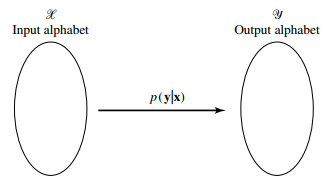
\includegraphics[width=0.6\linewidth]{./channel_model.PNG}\\[1cm]
\end{center}
\begin{equation}
    p(y|x) = Q.(\sqrt{\frac{2E_b}{N_0}})
\end{equation}


\par Write something here.\\
\section{Motivation}
\par Write something here.\\

\chapter{CHANNEL MODEL}
\begin{equation}
    p(y|x) = \prod_{i=1}^{n} p(y_i|x_i)
\end{equation}
\begin{equation}
    p(y|x) = Q.(\sqrt{\frac{2E_b}{N_0}})
\end{equation}
\begin{equation}
    \frac{1}{n}\sum_{i=1}^{n}x_i^2 <= P
\end{equation}


\chapter{CHANNEL CAPACITY}
\begin{equation}
    \binom{n}{n\epsilon}
\end{equation}
\par Denoting $\overline{\epsilon}=1-\epsilon$, Applying Sterling's approximation we have $n!\approx\sqrt{2\pi n}n^ne^{-n}$, $(n\epsilon)!\approx\sqrt{2\pi n\epsilon}(n\epsilon)^{n\epsilon}e^{-n\epsilon}$ and $(n\overline{\epsilon})!\approx\sqrt{2\pi n\overline{\epsilon}}(n\overline{\epsilon})^{n\overline{\epsilon}}e^{-n\overline{\epsilon}}$
\begin{equation}
    \begin{split}
    \binom{n}{n\epsilon} = &\frac{n!}{(n\epsilon)!(n\overline{\epsilon})!}
    \approx \frac{\sqrt{2\pi n}n^ne^{-n}}{\sqrt{2\pi n\epsilon}(n\epsilon)^{n\epsilon}e^{-n\epsilon}\sqrt{2\pi n\overline{\epsilon}}(n\overline{\epsilon})^{n\overline{\epsilon}}e^{-n\overline{\epsilon}}}\\
    = &\frac{1}{\sqrt{2\pi n\overline{\epsilon}}\epsilon^{n\epsilon}\overline{\epsilon}^{n\overline{\epsilon}}}
    \end{split}
\end{equation}
\par From above
\begin{equation}
    \frac{1}{n}\log_{2}\binom{n}{n\epsilon} \approx & -\frac{1}{2n}\log_{2}(2\pi n\epsilon\overline{\epsilon})-\epsilon\log_{2}\epsilon - \overline{\epsilon}\log_{2}\overline{\epsilon}
    \rightarrow & -\epsilon\log_{2}\epsilon - \overline{\epsilon}\log_{2}\overline{\epsilon} \text{as} n \rightarrow \infty
    = & H_b(\epsilon)
\end{equation}
\par When $n\rightarrow\infty$, $\binom{n}{n\epsilon}\approx2^{nH_b(\epsilon)}$
\par Using Sterling 's approximation
\begin{equation}
    \binom{n}{n\epsilon} \approx 2^{n.H_b(\epsilon)}
\end{equation}
\par Where $H_b(\epsilon) = -\epsilon.\log_{2}\epsilon-(1-\epsilon).\log_{2}(1-\epsilon)$

\begin{equation}
    M = \frac{2^{n.H(Y)}}{2^{n.H_b(\epsilon)}} = 2^{n.(H(Y)-H_b(\epsilon))}
\end{equation}

\begin{equation}
    R = \frac{\log M}{n} = H(Y) - H_b(\epsilon)
\end{equation}
\begin{equation}
    R = 1 - H_b(\epsilon)
\end{equation}

\par \textbf{Theorem[Noisy Channel-Coding Theorem]} .The capacity of a discrete-memoryless channel is given by
\begin{equation}
    C = \max_{p(x)}I(X;Y)
\end{equation}

\section{Gaussian Channel Capacity}
\par The input-output relation of a discrete-time Gaussian channel with power constraint is given by
\begin{equation}
    Y = X + Z
\end{equation}
where Z is zero-mean Gaussian random variable with variance $P_N$. When calculating the input power, applying the power constraint we have
\begin{equation}
    \frac{1}{n}\sum_{i=1}^{n}x_i^2\leq P
\end{equation}
For blocks of length \textit{n} at the input, the output and the noise we have
\begin{equation}
    \textbf{y=x+z}
\end{equation}
If n is large, we have
\begin{equation}
    \frac{1}{n}\sum_{i=1}^{n}z_i^2=\frac{1}{n}\sum_{i=1}^{n}(y_i^2-x_i^2)\leq P_N
\end{equation}
or
\begin{equation}
    ||y-x||^2 \leq nP_N
\end{equation}
It clearly that the above equation is having a form of an circle function, but because of the n-dimensions we have a sphere with a radius of $\sqrt{nP_N}$ and centered at x.
\par Due to the input power constraint and the independence of input and noise, the output power is the sum of input power and noise power
\begin{equation}
    \frac{1}{n}\sum_{i=1}^{n}y_i^2\leq P+P_N
\end{equation}
or
\begin{equation}
    ||y||^2\leq n(P+P_N)
\end{equation}
\par We interpret this as the output sequence would lie inside an n-dimensional hypersphere with $\sqrt{n(P+P_N}$ as radius and have center at the origin



\par The volume of a hypersphere can be computed 
\begin{equation}
    V_n = K_nR^n
\end{equation}
\begin{equation}
\begin{split}
    M = \frac{K_n(n(P_N+P)^{n/2}}{K_n(nP_N)^{n/2}}\\
    =(\frac{P_N+P}{P_N})^{n/2}\\
    =(1+\frac{P}{P_N})^{n/2}
\end{split}
\end{equation}

\begin{equation}
\begin{split}
    C = \frac{1}{n} \log M
    = \frac{1}{n} \frac{n}{2} \log(1 + \frac{P}{P_N})
    = \frac{1}{2} \log (1+\frac{P}{P_N})
\end{split}    
\end{equation}
\begin{equation}
    P_N = \int_{-W}^{+W}\frac{N_0}{2}df = WN_0
\end{equation}
\begin{equation}
    C = \frac{1}{2}\log (1 + \frac{P}{N_0W}
\end{equation}
\begin{equation}
    C = W\log (1 + \frac{P}{N_0W}
\end{equation}



\chapter{BOUND ON COMMUNICATION}
\begin{equation}
    \lim_{W\rightarrow\infty} C = \frac{P}{N_0}\log e = 1.44\frac{P}{N_0}
\end{equation}
\begin{equation}
    R < W\log (1 + \frac{P}{N_0W})
\end{equation}
\begin{equation}
    r < \log ( 1 + \frac{P}{N_0W})
\end{equation}
\begin{equation}
    r < \log(1 + r\frac{\varepsilon_b}{N_0})
\end{equation}
\begin{equation}
    \frac{\varepsilon_b}{N_0} > \frac{2^r -1}{r}
\end{equation}

\end{document}
here
